\chapter{Conclusion}
brief of conclusion

\section{Conclusion of Problems}
Tell about solving the problem

\section{Conclusion of Method}
Tell about solving using method

\section{Conclusion of Experiment}
Tell about solving in the experiment

\section{Conclusion of Result}
tell about result for purpose of this research.

\section{Yusniar Nur Syarif Sidiq/1164089}
\subsection{Pemahaman Teori / Yusniar Nur Syarif Sidiq / 1164089}

\begin{enumerate}

\item Jelaskan kenapa kata-kata harus dilakukan vektorisasi. Dilengkapi dengan ilustrasi atau gambar.
	\subitem Dikarenakan mesin hanya mampu membaca data dengan bentuk angka maka dari itu diperlukan vektorisasi kata atau bisa disebut dengan mengubah kata menjadi bentuk vektor agar mesin seolah-olah paham apa yang kita maksudkan. Kal inii saya memberikan ilustrasi sederhana, dimana ada sebuah data mengenai kucing, tikus, dan pulpen. Bagaimana cara mesin untuk membaca data tersebut ?, yaitu dengan cara dilakukannya vektorisasi kata. Fungsi dari vektorisasi itu sendiri ialah sebagai indentitas, misalnya di dalam dokumen kucing terdapat kata-kata yang sudah di vektorisasi dan hasilnya adalah 0.012,0.024,.....,0.300, pada dokumen tikus menghasilkan 0.015,0.026,....,0.0276, dan pada pulpen menghasilkan -0.191,...,-0.045. Data vektor tersebut merupakan identitas dari data kucing, tikus dan pulpen.Apabila nilai vektor cenderung sama, maka data tersebut memiliki similarity atau data yang memiliki konten kata yang sama akan tetapi berbeda dengan pulpen yang memiliki data vektorisasi minus, sehingga dapat disimpulkan pulpen memiliki konten kata yang berbeda. Dengan adanya vektorisasi tersebut maka mesin seolah-olah mengerti bahwa kucing dan tikus memiliki konten yang sama yaitu merupakan objek dari binatang sedangkan pulpen merupakan objek benda mati. Mengenai contoh gambarnya dapat dilihat pada figure \ref{YNC5-1}

	\begin{figure}[ht]
		\centering{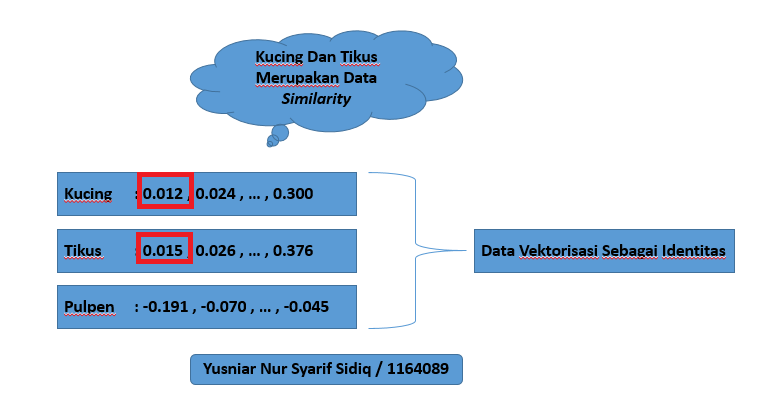
\includegraphics[scale=0.5]{figures/YN/Chapter5/Teori/YNC5-1.png}}
		\caption{Kata-Kata Hasil Vektorisasi}
		\label{YNC5-1}
	\end{figure}

\item Jelaskan mengapa dimensi dari vektor dataset google bisa sampe 300. Dilengkapi dengan ilustrasi atau gambar.
	\subitem Dikarenakan pada setiap dataset didalamnya memiliki identitas masing-masing yang menyebabkan jumlah vektor dataset google bisa sampe 300. Saya akan memberikan sebuah ilustrasi yang saya dapat yaitu bagaimana pembagian dataset pada google. Didalam dataset google tersebut memiliki beberapa objek yaitu spatula, cat, dan dog. Dimana ketiga dataset tersebut akan dilakukan proses perbandingan dataset sehingga diproleh hasil antara cat dan dog yaitu 76\% dikarekan pada dataset cat dan dog memiliki kesamaan data sedangkan untuk hasil perbandingan antara cat dan spatula yaitu 12\%. Mengapa lebih sedikit, dikarenakan data yang dimiliki oleh cat dan spatula tidak memiliki kesamaan data. Hal ini dapat membuktikan setelah dilakukan vektorisasi mesin jadi dapat membedakan mana dataset yang memiliki kesamaan dan mana yang bukan. Mengenai pengertian dan ikustrasi tersebut dapat kita liat kedalam bentuk figure \ref{YNC5-5}

	\begin{figure}[ht]
		\centering{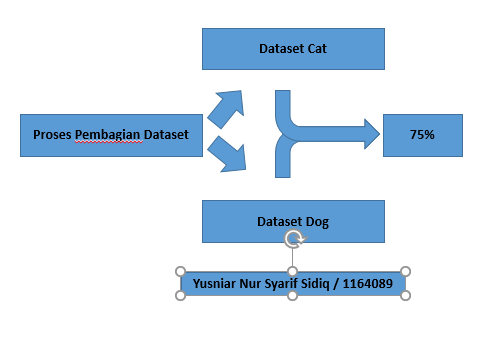
\includegraphics[scale=0.5]{figures/YN/Chapter5/Teori/YNC5-5.png}}
		\caption{Dataset Google}
		\label{YNC5-5}
	\end{figure}

\item Jelaskan konsep vektorisasi untuk kata. Dilengkapi dengan ilustrasi atau gambar.
	\subitem Konsep pada vektorisasi kata yaitu dimana kata tersebut merupakan sebuah hasil pengolahan kata dari sebuah kalimat-kalimat yang telah kita olah. Misalnya saat kita membuka sosial media dan terdapat banyak komentar didalamnya. Ada sebuah kalimat yang mengatakan \" Follow instagram aku yah teman-teman \" , dimana dalam kalimat tersebut memiliki kata kunci instagram dan kata tersebut akan dijadikan data training untuk mesin. Diamana nantinya mesin akan menampilkan kata-kata yang ada kaitannya dengan kata kunci tersebut. Figure \ref{YNC5-3} merupakan sebuah ilustrasi pada vektorisasi kata.

	\begin{figure}[ht]
		\centering{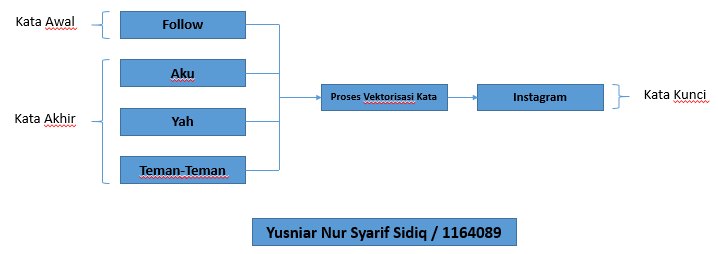
\includegraphics[scale=0.5]{figures/YN/Chapter5/Teori/YNC5-2.png}}
		\caption{Vektorisasi Kata}
		\label{YNC5-2}
	\end{figure}

\item Jelaskan konsep vektorisasi untuk dokumen. Dilengkapi dengan ilustrasi atau gambar.
	\subitem Sebenarnya konsep pada vektorisasi dokumen dan vektorisasi kata itu sama saja, hal yang membedakannya itu hanya proses awalnya. Dimana pada vektorisasi kata akan membaca kalimat per kalimat namun pada vektorisasi dokumen akan membaca keseluruhan kalimat yang terdapat pada sebuah dokumen yang nantinya kalimat-kalimat tersebut akan dipecah menjadia kata per kata. Pada figure \ref{YNC5-3} merupakan contoh ilustrasi sederhana.

	\begin{figure}[ht]
		\centering{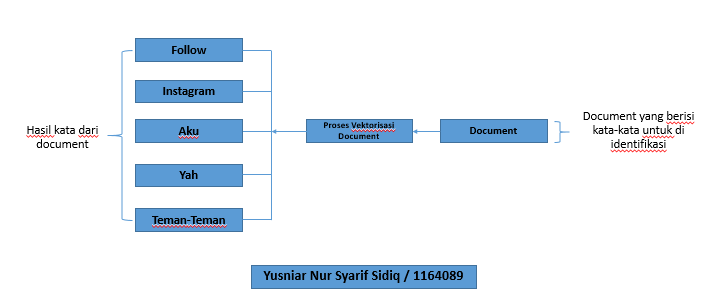
\includegraphics[scale=0.5]{figures/YN/Chapter5/Teori/YNC5-3.png}}
		\caption{Vektorisasi Document}
		\label{YNC5-3}
	\end{figure}

\item Jelaskan apa mean dan standar deviasi. Dilengkapi dengan ilustrasi.
	\subitem Mean merupakan nilai rata-rata dari suatu data. Mean dapat dicari dengan cara membagi jumlah data dengan banyak data sehingga diperoleh lah nilai rata-rata dari suatu data. Sedangkan standar deviasi merupakan sebuah teknik statistik yang digunakan dalam menjelaskan homogenitas kelompok. Contoh sederhananya dimana kita menjumpai dataset yang memiliki 10 data yang berbeda dan 5 atribut yang berbeda. Untuk memperolah nilai mean kita harus menghitung keseluruhan data tersebut lalu hasilnya akan dibagi dengan jumlah datanya. Setelah kita mendapatkan nilai mean maka kita bisa menghitung standar deviasi untuk memperoleh nilai statisknya.

\item Jelaskan apa itu skip-gram. Dilengkapi dengan ilustrasi atau gambar.
	\subitem Skip-gram merupakan sebuah teknik yang digunakan pada area speech processing yang dimana n-gram dibentuk lalu ditambah dengan tindakan skip. Misalkan ada sebuah kalimat yaitu \" I hit the tennis ball \", kita akan membuatnya menjadi skip gram 3 kata maka akan menjadi,
		\begin{itemize}
			\item I hit the
			\item Hit the tennis
			\item The tennis ball
		\end{itemize}
Figure \ref{YNC5-4} merupakan ilustrasi sederhana.
		\begin{figure}[ht]
		\centering{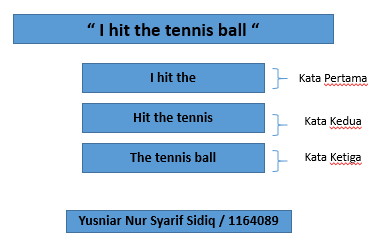
\includegraphics[scale=0.5]{figures/YN/Chapter5/Teori/YNC5-4.png}}
		\caption{Kata-Kata Hasil Vektorisasi}
		\label{YNC5-4}
	\end{figure}

\end{enumerate}

\section{Imron Sumadireja / 1164076}
\subsection{Teori}
\begin{enumerate}
\item Jelaskan kenapa kata-kata harus dilakukan vektorisasi. Dilengkapi dengan ilustrasi \par
Karena untuk mengetahui presentase kata yang sering muncul dalam setiap kalimatnya, yang berguna untuk menetukan kata kunci, serta untuk memberikan kemudahan bagi mesin untuk mempelajari kata yang bentuk aslinya serupa namun tak sama seperti bebek dan ayam. Selain itu fungsi dari vektorisasi kata ini untuk membaca setiap kata-katanya dengan merubah kata menjadi sebuah angka atau identitas itu sendiri \ref{vek1}.
		\begin{figure}[ht]
		\centerline{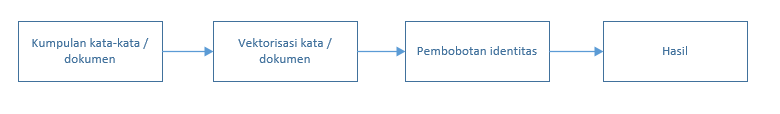
\includegraphics[width=0.5\textwidth]{figures/im/vek1.png}}
		\caption{Ilustrasi Vektorisasi Kata.}
		\label{vek1}
		\end{figure}

\item Jelaskan mengapa dimensi dari vektor dataset google bisa sampai 300. Dilengkapi dengan ilustrasi \par
Karena pada masing-masing objek itu memiliki identitas tersendiri, contoh sederhananya. Pada dataset google ini memiliki 3 buah objek diantaranya, cat, dog, dan spatula. Lalu dari masing-masing objek itu dibandingkan datasetnya antara cat dan dog lalu cat dan spatula. Hasil yang didapatkan untuk cat dan dog itu sekitar 76\% sedangkan untuk cat dan spatula itu memiliki presentase 12\% itu artinya bahwa mesin dapat membedakan objek yang hampir serupa namun tak sama. Untuk ilustrasi sederhananya bisa dilihat pada gambar \ref{vek2}.
		\begin{figure}[ht]
		\centerline{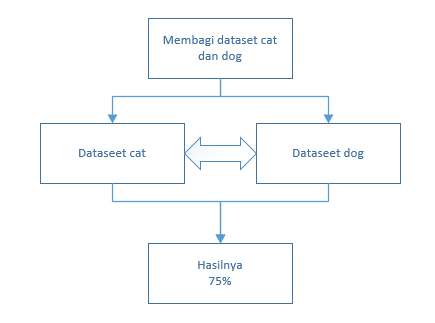
\includegraphics[width=0.5\textwidth]{figures/im/vek2.png}}
		\caption{Ilustrasi Vektorisasi Dataset Google.}
		\label{vek2}
		\end{figure}

\item Jelaskan konsep vektorisasi untuk kata. Dilengkapi dengan ilustrasi \par
Konsep untuk vektorisasi kata ini sama halnya dengan kita input suatu kata pada mesin pencari. Lalu hasilnya akan mengeluarkan berupa referensi mengenai kata tersebut. Jadi data kata tersebut didapatkan dari hasil pengolahan pada kalimat-kalimat sebelumnya yang telah diolah. Contoh sederhananya pada kalimat berikut ( Please subscribe my channel thank you guys ), pada kalimat tersebut terdapat konteks yakni channel, kata tersebut akan dijadikan data latih untuk mesin. Jadi ketika kita inputkan kata channel, maka mesin akan menampilkan keterkaitannya dengan kata tersebut. Ilustrasinya bisa dilihat pada gambar berikut \ref{vek3}.
		\begin{figure}[ht]
		\centerline{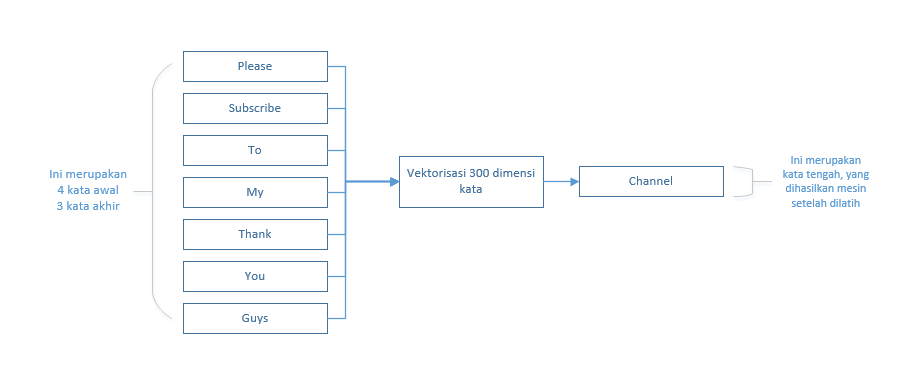
\includegraphics[width=0.5\textwidth]{figures/im/vek3.png}}
		\caption{Ilustrasi Vektorisasi Kata.}
		\label{vek3}
		\end{figure}

\item Jelaskan konesep vektorisasai untuk dokumen. Dilengkapi dengan ilustrasi \par
Sama halnya dengan vektorisasi kata, yang membedakan hanya pada proses awalnya. Untuk vektorisasi dokumen ini, mesin akan membaca semua kalimat yang terdapat pada dokumen tersebut, lalu kalimat yang terdapat pada dokumen akan di pecah menjadi kata-kata. Untuk ilustrasinya dapat dilihat pada gambar berikut \ref{vek4}.
		\begin{figure}[ht]
		\centerline{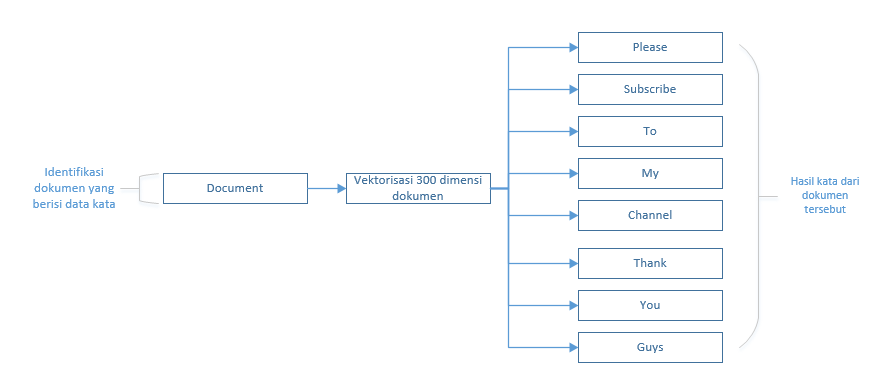
\includegraphics[width=0.5\textwidth]{figures/im/vek4.png}}
		\caption{Ilustrasi Vektorisasi Dokumen.}
		\label{vek4}
		\end{figure}

\item Jelaskan apa mean dan standar deviasi. \par
Mean merupakan nilai rata-rata. Untuk mendapatkan mean ini kita tinggal menjumlahkan data yang tersedia lalu dibagi dengan banyaknya data tersebut. Sedangkan standar deviasi adalah nilai statistik yang digunakan untuk menentukan bagaimana sebaran data dalam sampel, dan seberapa dekat titik data individu dengan rata-rata nilai sampel.

\item Jelaskan apa itu skip-gram. Dilengkapi dengan ilustrasi \par
Skip-gram sama halnya dengan vektorisasi kata, namun untuk skip-gram ia dibalik prosesnya. Yang sebelumnya dari kalimat lalu di olah untuk menemukan salah satu kata, kali ini dari keyword tersebut akan diolah menjadi suatu kalimat yang memiliki keterkaitannya dengan keyword tersebut. Ilustrasinya bisa dilihat pada gambar berikut \ref{vek5}.
		\begin{figure}[ht]
		\centerline{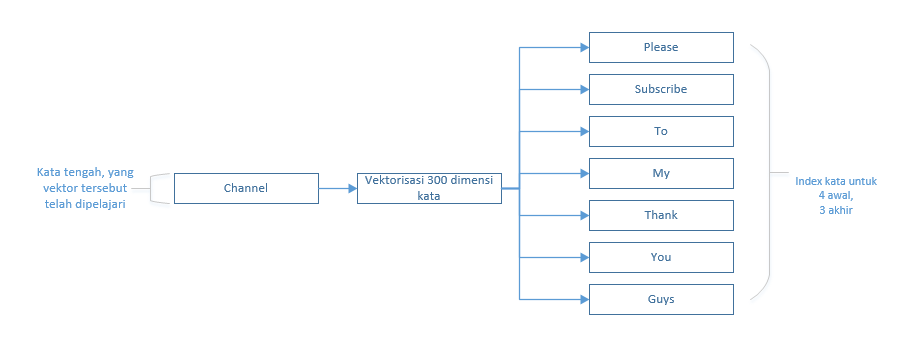
\includegraphics[width=0.5\textwidth]{figures/im/vek5.png}}
		\caption{Ilustrasi Skip-Gram.}
		\label{vek6}
		\end{figure}

\end{enumerate}